\documentclass{article}
\usepackage{graphicx}
\usepackage{amsmath}
\usepackage{hyperref}
\usepackage{float}
\usepackage{xcolor}
\usepackage{enumitem}
\usepackage{hyperref}
\usepackage{mathtools}

\begin{document}

\title{Solutions to hw2 homework on Convex Optimization https://web.stanford.edu/class/ee364b/homework.html}
\author{Andrei Keino}
\maketitle

\section*{2.1 (8 points, 1 point per question)} 
Let $f$ be a convex function with domain in $R^n.$ 
We fix $x \in \bf{int \; dom}\; f  $ and $d \in R^n.$
Recall the definition of the directional derivative of $f$
at $x$ along the direction $d$
$$
f'(x, d) = \lim_{t \rightarrow 0} \frac{f(x + td) - f(x)}{t}
$$
In this question we aim to show that $f'(x, d)$ exists and is finite, and that we have the following relationship 
between $\partial f(x)$  and $f'(x, d),$
$$
f'(x, d) = \sup_{g \in \partial f(x)} g^T d
$$
\\

(a) Show that the ratio $\frac{f(x + td) - f(x)}{t}$ is a nondecrasing function of $t > 0.$ Deduce that $f'(x, d)$
exists and is either finite or equal to $- \infty.$ \\
We know from the lectures that, since $x \in \bf{int \; dom \;} f,$ the subdifferential set $\partial f$ is non - empty, convex and compact.
\\

Solution:\\

\textbf{Proof of non - decreasing.}
Definition of subgradient is
$$
f(z) \geq f(x) + g^T(z - x)
$$
let $z = x + td;$ then
$$
f(x + td) \geq f(x) + g^T(x + td - x)
$$
or 
$$
f(x + td) - f(x) \geq t g^T d
$$
dividing both part of the inequality by $t$ (as $t > 0,$
we can do it) gives

$$
\frac{f(x + td) - f(x)}{t} \geq g^T d
$$
as the right - hand side of the equation is not depends of $t,$ differentiating by $t$  gives
$$
\partial \frac {\frac{f(x + td) - f(x)}{t}} {\partial t} \geq 0
$$


\textbf{As the $\frac{\partial f'(x, d}{\partial t} \geq 0,$ it means the function $f'(x, d)$ is nondecreasing by variable $t.$ }

\textbf{Proof of possible equality to $- \infty.$}\\
The definition of convexity: \\

$$
f(\theta x + (1 - \theta) y)) \leq 
\theta f(x) + (1 - \theta) f(y)
$$
where $0 < \theta < 1.$ \\
let $t = 1 - \theta,$ $0 < t < 1.$
then
$$
f((1 - t) x + t y)) \leq 
(1 - t)f(x) + tf(y)
$$
or
$$
f(x + t (y - x))) \leq 
f(x) + t(f(y) - f(x))
$$
as we can choose $y$ any of the point in domain $f,$ we can set $d = y - x.$ Then
$$
f(x + t d) \leq 
f(x) + t(f(y) - f(x))
$$
or
$$
f(x + t d) - f(x)\leq 
t(f(y) - f(x))
$$
or
$$
\frac{f(x + t d) - f(x)}{t}\leq 
f(y) - f(x)
$$
\textbf{As $f(x)$ can be equal to $\infty$ on the domain of $f$, so
$f'(x, d) = \frac{f(x + t d) - f(x)}{t}$ can be less or equal than (for the infinity with sign minus it means strictly equal) $- \infty$ on the domain of $f.$} This means that $f'(x, d)$ can be equal to $- \infty$ on domain of $f.$\\

(b) Let $g \in \partial f(x).$ Show that 
$f'(x, d) \geq g^T d.$ Deduce that $f'(x, d)$ is finite and $f'(x, d) \geq \sup_{g \in \partial f(x)} g^T d.$ \\

Solution:\\
We already shown that 
$$f'(x, d) \geq g^T d$$
in part (a).
We also shown in part (a) that 
$$
\frac{f(x + t d) - f(x)}{t}\leq 
f(y) - f(x)
$$
Second upper inequality means that  $f'(x, d)$ is bounded from upper side (i.e it can't be equal to $\infty$), it means  its value is finite. \\
As the first of upper inequalities is correct $\forall$ subgradients in domain of $f,$ it means, that it is correct for  the supremum of these subgradients in domain $f.$ It means that 
$$f'(x, d) \geq \sup_{g \in \partial f(x)} g^T d.$$
\\

In the remaining part of this question, we will establish the converse inequality $f'(x, d) \leq \sup_{g \in \partial f(x)} g^T d,$ by showing the existence of a subgradient $g^* \in \partial f(x), $ such that 
$f'(x, d) \leq g^{*T} d.$ We introduce two following sets
\begin{align*}
	C_1 &= \{(z,t) \; |\; z \in \mathbf{dom} f, \; f(z) < t \} \\
	C_2 &= \{(y, v) \; | \; y = x + \alpha d, \;
	v = f(x) + \alpha f'(x, d), \; \alpha \geq 0 \}
\end{align*}

(c) Prove that $C_2$ and $C_2$ are nonempty, convex and disjoint.\\

Solution: \\

$C_1$ is the epigraph of the convex function, therefore 
it is nonempty and convex.

$C_2$ is the nonempty set, because it have at least one point, which corresponds to $\alpha = 0,$ $y = x,$ $v = f(x).$ It is also a convex set, because 
$C^1_2 = \{y\;| \;y = x + \alpha d\}$ is a convex set as it is translated domain of $f$ which is a convex set
and $C^2_2 = \{v\;| \; 
v = f(x) + \alpha f'(x, d), \; \alpha \geq 0 \}$ is either 
a straight line or a beam or a segment. \\

Proof of disjointedness: \\
We should show that there is exists a nonzero vector 
$(a, \beta) \in R^n \times R$ such as
$$
a^T(x + \alpha d) + \beta (f(x) + \alpha f'(x, d)) \leq
a^T z + \beta w
$$
for all $\alpha \ geq 0, $ $z \in \mathbf{dom} f,$ 
and $f(z) < w.$
\\
Solution:
As we shown earlier, 
$$
f'(x, d) \leq f(y) - f(x)
$$
where $x, y \in \mathbf{dom} f.$ As $x, y$ can be any points in domain $f,$ it follows that\\
$$
f'(x, d) \leq \min_{z \in \mathbf{dom} f }(f(z)) - 
\max_{z \in \mathbf{dom} f}(f(z))
$$
Lets just derive equation for $\beta.$

$$
\beta (f(x) + \alpha f'(x, d) - w) \leq 
a^T(z - x - \alpha d)
$$
or
$$
\beta \leq \frac{a^T (z - x - \alpha d)}
{f(x) + \alpha f'(x, d) - w}
$$

I don't know how to solve items (e) - (g) \\\

(h) Let $A \in R^{m\times n},$ $b \in R^m,$ $\lambda > 0,$ 
and fix a direction $d \in R^n.$ Consider the function 
$\frac{1}{2} ||Ax - b||^2_2 + \lambda ||x||_1.$ Compute 
$f'(0, d).$ Remark: you can either compute it
directly by using the definition of the directional derivative, or, use the variational
formula $f'(0, d) = \sup_{g \in \partial f(0)} g^T d.$
\\

Solution: \\ \\
$
\nabla ||x||_1 = sign(x)
$\\

$\nabla ||Ax - b||^2_2 = \nabla((Ax - b)^T (Ax - b)) = 2(Ax - b)^T A
$\\ \\
see\url{ https://math.stackexchange.com/questions/606646/matrix-derivative-ax-btax-b}
and 
\url{
http://www.math.uwaterloo.ca/~hwolkowi//matrixcookbook.pdf
}

So, \\
$
\nabla (\frac{1}{2} ||Ax - b||^2_2 + \lambda ||x||_1) = 
2(Ax - b)^T A + \lambda sign(x)
$
\\ \\
Then \\
$$
f'(0, d) = d^T ((Ax - b)^T A + \lambda [-1, 1]_n) 
$$
where $ [-1, 1]_n$ is a vector in $R^n$ with component values in range \\
$-1 \leq x_i \leq 1, \; i \in {1, \dots , n}.$

\section*{2.2 (4 Points)} 
In this question, we will show that a subgradient of the function \\ 
$h(x) = \min_{z \in C} ||x - z||_2$ is 
$$
g = \frac{x - z^*}{||x - z^*||_2}
$$
where $C$ is a compact set in $R^n,$ $x$ is a given point in $R^n,$ which does not belong to $C,$ and \\ 
$z^* = P_C(x) := \operatorname*{arg\,min}_{z \in C}||x - z||_2$ denotes the Euclidean projection of $x$ onto
$C$ (which exists and is unique). \\

(a) (0.5 point) Use the fact that 
$||x - z||_2 = \max_{u:||u||_2 \leq 1} u^T(x - z)$ to transform the minimization problem ]
$h(x) = \min_{z \in C} ||x - z||_2$ into the following saddle point problem
$$
\min_{z \in C} \max_{u:||u||_2 \leq 1} u^T(x - z)
$$
\\ Solution: \\

We get it by substituting expression $\max_{u:||u||_2 \leq 1} u^T(x - z)$ instead the expression $||x - z||_2.$\\

(b) (2 points) Now, we will use (a simple version of) the Sion's minimax theorem, which can be stated as follows. \\
Let $X \subseteq R^n, $ $Y \subseteq R^n, $ be compact and convex sets. Let $f$ be a real valued function on 
$X\times Y$ such that \\
- $f(x, \cdot) $ is continuous and concave on $Y, $ 
$\forall x \in X.$ \\
- $f(\cdot, y) $ is continuous and convex on $X, $ 
$\forall y \in Y.$ \\

Then, we have \\
$\min_{x \in X} \max_{y \in Y} f(x, y) = \max_{y \in Y} \min_{x \in X}  f(x, y)$ \\ \\
Further, there exists a (saddle) point 
$(x^*, y^*) \in X \times Y $ such that 
$$
f(x*, y*) = \min_{x \in X} f(x, y^*) = 
\max_{y \in Y} f(x*, y) = \min_{x \in X} \max_{y \in Y} f(x, y) = \max_{y \in Y} \min_{x \in X}  f(x, y)
$$
Apply Sion's minimax theorem to conclude that
$$
\min_{z \in C} \max_{u:||u||_2 \leq 1} u^T(x - z) = 
 \max_{u:||u||_2 \leq 1} \min_{z \in C} u^T(x - z)
$$
Define $u^* = \frac{x - z^*}{||x - z^*||_2}.$ Show that 
$(z^*, u^*)$ is a saddle point of the above minimax problem.
\\

Solution: \\
$C$ is compact and convex. $u$ defined on the closed sphere $S$ of unity radius, therefore its domain is compact and convex also. The function $f(u, z) = u^T(x - z)$ is linear 
in sense of both $f(z, \cdot)$ on $C$ and $f(\cdot, u)$ 
on $S.$ It means that it is concave and convex in both cases. So, applying Sion's minimax theorem  we have:\\
$$
\min_{z \in C} \max_{u:||u||_2 \leq 1} u^T(x - z) = 
\max_{u:||u||_2 \leq 1} \min_{z \in C} u^T(x - z)
$$
where ${f(z, u) = u^T(x - z)}$
and there exist a saddle point $(z^*, u^*)$ in $C \times S$
such that 
$$
f(z^*, u^*) = \min_{z \in C} f(z, u^*) = 
\max_{u \in S} f(z^*, y) = \min_{z \in C} \max_{u \in S} f(z, u) = \max_{z \in C} \min_{u \in S}  f(z, u)
$$

define $u^* = \frac{x - z^*}{||x - z^*||_2}.$ It is evident, that $u^*$ is the solution of the problem 
$\max_{u:||u||_2 \leq 1} u^T(x - z).$ Also, this is evident, that the point $z^*$ is the solution of the problem 
${z^* = P_C(x) := \operatorname*{arg\,min}_{z \in C}
	u^T(x - z)_2}.$ 
Then, by Sion's theorem the point 
${(z^*, u^*): \, f(z^*, u^*)} = \min_{z \ in C} f(z, u^*),$
where ${f(z, u*) = u^{*T}(x - z)}$
is a saddle point of the problem 
$$
\min_{z \in C} \max_{u \in S} u^T(x - z)_2.
$$
\\

(c) (1.5 points) Using the 'max-min' representation of $h(x)$, compute a subgradient of $h$ at $x$.
\\

Solution:
$$
g = u \nabla (x - z^*) = u = \frac{x - z^*}{||x - z^*||_2}
$$

\section*{2.3 (4 points)} 

For this question, you need to submit your code in addition to any description
of your algorithm. Let $\Sigma$ be an $n \times n$ diagonal matrix with entries 
$\sigma_1 \geq \dots \geq \sigma_n$ and $y$ a given vector 
in $R^n.$ Consider the compact convex sets 
$\mathcal{E} = \{z \in R^n|\; 
||\Sigma ^{\frac{1}{2} } z||_2 \leq 1\}$
and $B=\{z \in R^n|\; ||z-y||_{\infty} \leq 1 \}.$ \\

(a) (2 points) Formulate an optimization problem and propose an algorithm in order to find a point
$x \in \mathcal{E} \cap B.$ You can assume that $\mathcal{E} \cap B$ is not empty. Your algorithm must be provably converging (although you do not need to prove it and you can simply refer to the lectures' slides).\\

Solution:\\
As $\Sigma$ is a diagonal matrix, 
$||\Sigma ^{\frac{1}{2} } z||_2 = 
||\lambda^T z||_2,$ where $\lambda \in R^n, $ and 
$\lambda = (\sqrt{\sigma_1}, \dots, \sqrt{\sigma_n}).$ It means that $\mathcal{E}$ is an ellipse in $R^n$ with the center in the point $(0)^n$. The set $B $ is a cube in $R^n$ with edge length 2 and with the center at the point $y.$ \\

%C:\!Convex_Optimization\ConvexOptimizationII\materials\lsocoee364b\02_subgrad_method_notes.pdf
% page 11

% Finding a point in the intersection of convex sets

% Finding a point in the intersection of convex sets

% C:\! Convex_Optimization\! ee346b_homework\hw1_subgrad_method_matlab\subgrad_method_dual_prob.m -- solving dual problem using proj. subgrad method 
Reference to lecture slides - Finding a point in the intersection of convex sets, sildes to 2-nd lection, p. 18.
%C:\! Convex_Optimization\ConvexOptimizationII\materials\lsocoee364b\02-subgrad_method_slides.pdf, p. 18

ecludian projection of point to ellipse
https://www.geometrictools.com/Documentation/DistancePointEllipseEllipsoid.pdf

https://math.stackexchange.com/questions/1775174/distance-function-of-the-ellipse-in-mathbbrn
\\

ecludian projection of point to cube

https://math.stackexchange.com/questions/3390029/projecting-a-point-onto-a-hypercube

a version of the alternating projections algorithm

An algorithm himself can be the following: \\

1. Begins from the point $x^{(0)} = 0^n,$ $x^{(0)} \in \mathcal{E}, $ and then applying the alternate projection method to this point and sets $\mathcal{E}$ and $B,$ i.e.  we are calculating the $x^{(1)} = P_B(x^{(0)}),$ $x^{(2)} = P_{\mathcal{E}}(x^{(1)}),$ $x^{(3)} = P_B(x^{(2)}),$ and so on. We are checking also if the point $x^{(k)} $ is in the both sets on each step. As the both sets are closed and
have intersection by the task, we have a guarantee, that we eventually will get a solution of the task. \\ 

(b) (2 points) Implement your algorithm with the following data: $n = 2,$ $y = (7/4, 0),$
$\sigma_1 = 1,$ $\sigma_1 = 0.5$ and $x = (0, 4).$ Plot the objective value of your optimization problem versus the number of iterations.

https://www.geometrictools.com/Documentation/DistancePointEllipseEllipsoid.pdf \\

The rectangle vertices are $\{(-1/4, 2), (1/4, -2), (15/4, 2), (15/4, -2])\}, $ the ellipse equation is $x^2 + y^2 / 2 \leq 1.$\\

Coordinates of the point found by the algorithm are 
$(0,  1.4142)$, the code is in the file \verb!2_3_b_solution.py!.

\begin{figure}[H]
	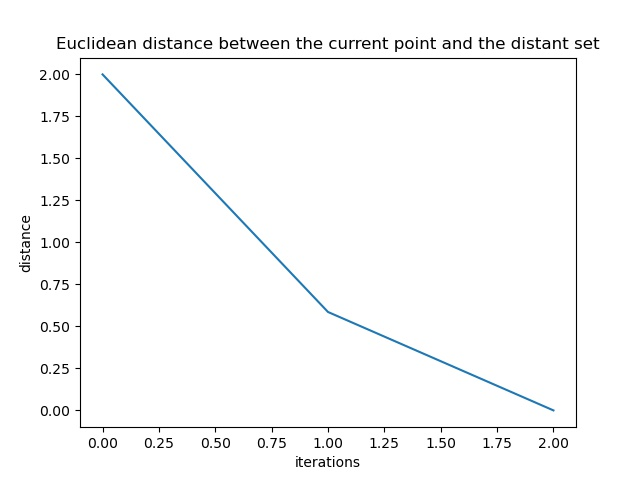
\includegraphics[width=\linewidth]{2_3_b_fig.jpeg}
	\caption{Euclidean distance between the current point and the distant set.}
	\label{fig:2_3_b_fig}
\end{figure}

\section*{2.4 (4 points)} 
Consider the optimization problem

\begin{align*}
	minimize & && 
	\bigg \{ f(x_1, \dots, x_j) \coloneqq
	\frac{1}{2} \lVert b - \sum_{j = 1}^{J} 
	A_j x_j \rVert_2^2 
	+ \lambda \cdot  \lVert \sum_{j = 1}^{J} 
	x_j^2 \rVert_2
	\bigg \},
	\\
\end{align*}
with variable $x_1, \dots, x_J \in R^n, $ and 
problem data $A_1, \dots, A_J \in R^{m \times n}, $ 
$b \in R^m,$ and $\lambda > 0.$ We will apply the subgradient method. \\

(a) (2 points) Show that the subgradient method with Polyak's step length updates the current point to a point at which the first order (linear) approximation has
value $f^*$ (optimal value).


\end{document}